\chapter{TypeScript}
JavaScript jest technologią, która od lat służy programistom do wzbogacania interfejsów stron internetowych o dynamikę. Dzisiaj JavaScript postrzegany jest jako technologia, która sprawia programistom wiele problemów. Wynika to przede wszystkim ze składni języka, braku mechanizmu typowania oraz niespotykanej nigdzie indziej  uproszczonej metodzie tworzenia hierarchii klas. Efekt ten jest spowodowany faktem, iż w momencie powstawania języka JavaScript, panowało przeświadczenie, iż nie będzie służył on do tworzenia dużych, kompletnych aplikacji. Postawiono zatem na prostotę rozwiązania. Dzięki niej programista jest w stanie szybko osiągnąć zamierzony cel niewielką ilością kodu.

\begin{figure}[h]
	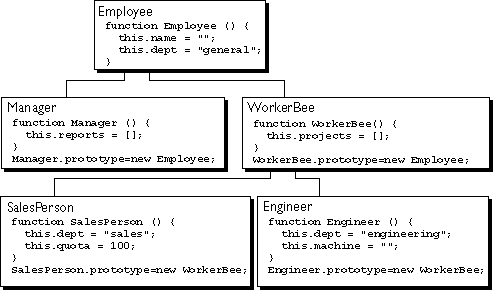
\includegraphics[width=140mm]{./img/javascript-inheritance.png}
	\caption{Mechanizm dDzisiaj rziedziczenia z wykorzystaniem obiektu prototype}
	\label{fig:javascript-inheritance}
\end{figure}

Rozwój aplikacji internetowych oraz przeglądarek pokazał, iż tworzenie bogatego interfejsu aplikacji daje wiele korzyści. JavaScript z biegiem lat nabierał znaczenia, gdyż coraz więcej przeglądarek wspierało tę technologię. W roku 1996 w oparciu o ten język został stworozny standard o nazwie ECMAScript, który obsługiwany jest dziś przez wszystkie przeglądarki. 

Programowanie interfejsów aplikacji internetowych doszło zatem do punktu, w którym programiści zmuszeni są używać JavaScript do tworzenia dużych aplikacji. Stało się to pomimo faktu, iż technologia ta została zaprojektowana do innego celu. Odpowiedzią na ten problem jest język TypeScript autorstwa Microsoftu.

\section{Cechy technologii}
Język TypeScript składa się z dwóch elementów - języka oraz kompilatora. Oba z nich są projektami na licencji OpenSource dostępnymi dla każdego. Aby lepiej zrozumieć możliwości technologii należy zapoznać się z następującymi faktami na jej temat:
\begin{itemize}
\item Język TypeScript jest kompilowany do języka JavaScript. Oznacza to, że poza kilkoma dodatkowymi słowami kluczowymi wystarczy znajomość JavaScript'u do posługiwania się TypeScript'em. 
\item Każdy fragment kodu napisany w JavaScript może zostać użyty do rozwoju klas w języku TypeScript. Dzięki temu możliwe jest wykorzystanie popularnych bibliotek takich jak jQuery, MooTools, itp. Społeczność regularnie dostacza pliki TypeScript, które zawierają definicje typów obiektów używanych przez różne biblioteki. Pozwala  to na wygodniejsze stosowanie ich zgodnie z zasadami języka TypeScript. 
\item Kompilator TypeScript'u jest zawarty w jednym pliku JavaScript i może zostać dołączony do każdego środowiska. Technologia nie posiada maszyny wirtualnej i nie ma planów na jej rozwój.
\end{itemize}
